% The `linenumber` option is necessary for ease of reviewer referencing



\documentclass[linenumber]{jdsart}

\volume{0}
\issue{0}
\pubyear{2026}
\articletype{research-article}
\doi{}

%startlocaldefs
%% Put your local definitions here

% local macros
%\newtheorem{thm}{Theorem}
%\newtheorem{prop}{Proposition}
%\newtheorem{cor}{Corollary}
%\newtheorem{lem}{Lemma}

%\theoremstyle{remark}
%\newtheorem{defn}{Definition}
%\newtheorem{rem}{Remark}
%\newtheorem{exmp}{Example}
%\newtheorem{note}{Note}

%endlocaldefs
\usepackage{tikz}
\usetikzlibrary{arrows.meta,calc}
\usepackage{xcolor}
\usepackage{graphicx}
\usepackage{placeins}

% TODO-VERIFY: Working draft intentionally retains verification comments and placeholders.
% Do not remove script/code evidence notes until the public-release repo, analysis
% scripts, notebooks, generated artifacts, manuscript tables, and figure assets are finalized.

\definecolor{figbg}{RGB}{245,247,251}
\definecolor{figdark}{RGB}{39,49,66}
\definecolor{figmid}{RGB}{95,111,141}
\definecolor{figblue}{RGB}{31,119,180}
\definecolor{figedge}{RGB}{53,92,125}
\definecolor{figlight}{RGB}{199,209,223}

\begin{document}



\begin{frontmatter}

\title{A Statistical Workflow for Interpretable Reduced-Form Surrogates from Large Simulators: A Case Study with the Bioenergy Scenario Model}
\runtitle{Reduced-Form Surrogates for Large Simulators}
%\title{\thanksref{t1}}
%\thankstext[id=t1]{}

\author[1]{\inits{D.}\fnms{Dylan}~\snm{Hettinger}\thanksref{t1}\ead{dylan.hettinger@nlr.gov}}
\author[2]{\inits{S.}\fnms{Steve}~\snm{Peterson}\ead{steve@evans-peterson.com}}
\author[1]{\inits{C.}\fnms{Colby}~\snm{Smith}\ead{colby.smith@nlr.gov}}
\author[1]{\inits{E.}\fnms{Emily}~\snm{Newes}\ead{emily.newes@nlr.gov}}

\thankstext[type=corresp,id=t1]{Corresponding author.}

\address[1]{\institution{National Laboratory of the Rockies (NLR)}, \cny{Golden, Colorado, USA}}
\address[2]{\institution{[Steve Peterson affiliation]}, \cny{[City, State, USA]}}

%\runtitle{}  %use if necessary to change auto-generated
%\runauthor{} %use if necessary to change auto-generated

%\dedicated{}

\begin{abstract} % avoid notations; avoid citations; no exceeding 250 words
% TODO-VERIFY: Confirm all abstract numbers against the final public-release artifacts:
% 20,000 runs; 160 inputs; 635 time-series outputs; 23,495 scalar responses;
% 10\% holdout; macro nRMSE 0.0445; and final support 340 = 61 + 242 + 37
% representing 62 unique original inputs.
Large scientific simulators can create input--output problems that are too large for routine sensitivity analysis, scenario screening, or downstream reuse. We present a staged workflow for constructing an interpretable reduced-form surrogate for this setting. The workflow reserves an external holdout set before any adaptive modeling, screens exogenous drivers with permutation-calibrated sensitivity measures, enriches the feature library with detected pairwise interactions and one-variable transformations, uses penalized regression on reduced response coordinates for support recovery, and fits a final ordinary least squares model on train-standardized selected predictors and train-standardized outputs. Predictions are then returned to the original output scale. We demonstrate the workflow on the Bioenergy Scenario Model, a deterministic system dynamics model of U.S. biofuels deployment. In the reported case study, 20,000 simulator runs, 160 exogenous inputs, and 635 annual time-series outputs flattened to 23,495 scalar responses were reduced to a final surrogate with holdout macro nRMSE of 0.0445. The exported model retained 340 predictors: 61 main effects, 242 pairwise interactions, and 37 one-variable transformations representing 62 unique original inputs. The result is an explicit algebraic surrogate whose selected support, coefficient matrices, preprocessing rules, and validation diagnostics can be inspected outside the original simulator.
\end{abstract}

\begin{keywords} % Alphabetical; not to repeat anything in the title
\kwd{algebraic metamodeling}
\kwd{feature selection}
\kwd{high-dimensional regression}
\kwd{multivariate output}
\kwd{penalized regression}
\kwd{principal component analysis}
\kwd{sensitivity screening}
\end{keywords}

\end{frontmatter}



\section{Introduction}
\label{sec:introduction}

Large simulators now create a class of statistical problems in which the challenge is not simply prediction from expensive runs. The more practical challenge is often to compress a high-dimensional input--output map into a reduced form that is computationally cheap, portable, and explicit enough for subsequent scientific analysis. In this setting, the central task is to move from a large-data simulator regime \citep{Donoho2017} to a statistically manageable high-dimensional reduced-form regime \citep{Wainwright2019} without losing the structure needed for prediction, explanation, and reuse \citep{Shmueli2010}.

The statistical foundation for this problem comes from the design and analysis of computer experiments \citep{SacksEtAl1989,SantnerWilliamsNotz2018} and surrogate modeling for complex simulators \citep{Gramacy2020}. Gaussian process emulators are a standard choice for expensive computer experiments and calibration problems \citep{KennedyOHagan2001,Gramacy2020}. Polynomial chaos expansions provide another route by representing model outputs in an orthogonal polynomial basis and, in some settings, enabling sensitivity indices to be computed from expansion coefficients \citep{Sudret2008}. Sparse polynomial chaos expansions reduce this burden when only a subset of polynomial terms is needed \citep{BlatmanSudret2011}. Active subspaces instead seek low-dimensional directions in the input space that explain dominant response variation \citep{Constantine2015}. These approaches are powerful, but they do not by themselves solve the particular problem targeted here: producing a named algebraic support and coefficient bundle that maps documented exogenous simulator inputs to thousands of documented scalar outputs.

A separate line of work in statistics and interpretable machine learning emphasizes additive representations \citep{HastieTibshirani1990}, sparse linear models \citep{Tibshirani1996}, hierarchical interaction structures \citep{BienTaylorTibshirani2013}, and model classes whose structure can be communicated directly rather than explained post hoc \citep{Rudin2019,AllenGanZheng2024}. The workflow proposed here sits at the intersection of these traditions. It uses calibrated screening, structured feature discovery, and sparse reduction to compress a large simulator problem into a smaller statistical representation, but it deliberately ends in an algebraic reduced form rather than a black-box emulator.

Global sensitivity analysis provides an important comparison point because it asks how variation in model outputs is attributable to variation in inputs, and it is widely used in environmental and systems modeling for uncertainty assessment, diagnostic evaluation, dominant-driver analysis, and robust decision support \citep{PianosiEtAl2016,IoossLemaitre2015}. Screening methods such as Morris designs can identify important factors with fewer runs than full variance decompositions \citep{Morris1991}, while variance-based and moment-independent measures provide richer importance summaries when the scientific target is input influence \citep{Sobol1993,Borgonovo2007,SaltelliEtAl2010}. The present workflow is complementary rather than a replacement. The difficulty in the motivating case is that even relatively efficient screening becomes awkward when hundreds of candidate inputs must be related to tens of thousands of scalar outputs, and when the desired deliverable is not only a ranking of inputs but a reusable multivariate input--output map. The proposed workflow therefore uses sensitivity ideas as part of a broader reduction pipeline: first identify a manageable external interface and selected support, then fit an explicit surrogate that can support prediction, scenario exploration, targeted sensitivity analysis, and coupling to other workflows \citep{RattoEtAl2012,PianosiEtAl2016,SaltelliEtAl2019}.

This article is a workflow paper. The contribution is a reproducible data-science design for converting a high-dimensional simulator interface into an explicit reduced-form model. The workflow separates the problem into distinct stages: defining an external input--output interface, reserving a holdout set before any adaptive modeling, constructing an algebraic feature library, conditioning outputs for discovery, screening effects with calibrated null references, discovering structured interactions and curvature, recovering a sparse support, and fitting a final ordinary least squares representation. The aim is not to claim a universal best surrogate model, but to make the reduction workflow auditable, portable, and testable.

The contribution is therefore methodological in design and empirical in demonstration. First, we formulate the surrogate task as a big-to-small statistical reduction problem in which both input-space and output-space growth must be controlled. Second, we present a staged workflow that links interface definition, screening, discovery, selection, estimation, prediction, validation, and interpretation into a coherent pipeline aimed at tractability and reproducibility. Third, we demonstrate in a demanding Bioenergy Scenario Model case study that this workflow can yield a reduced form with low holdout macro nRMSE while preserving an explicit input--output interface. The remainder of the article formalizes the generic problem, details the workflow, presents the case study and results, and then discusses scope, limitations, conclusions, and reproducibility.

\section{Problem Formulation}
\label{sec:problem}

For simulator run $i=1,\dots,n$, let
\[
u_i \in \mathbb{R}^d
\]
denote the vector of exogenous inputs. Stacking the model runs gives the raw input matrix
\[
U =
\begin{bmatrix}
u_1^{\top} \\
\vdots \\
u_n^{\top}
\end{bmatrix}
\in \mathbb{R}^{n \times d}.
\]
The components of $u_i$ may represent continuous variables, integer-valued settings, or binary indicators coded numerically as needed. The important restriction is not the input type, but the interface: the reduced form should depend only on exogenous quantities that can be sampled, documented, and reused outside the full simulator.

To extend the feature space, we construct an algebraic feature map
\[
\phi(u_i) \in \mathbb{R}^k,
\]
whose coordinates may include first-order terms, eligible pairwise interactions, and eligible simple nonlinear transformations of individual inputs. In the simplest form, this means starting with the original inputs, then augmenting them with terms such as $u_{ij}u_{i\ell}$ and $g(u_{ij})$ for a restricted set of transformations $g$ after screening and feature-discovery rules determine which terms are worth materializing. Stacking the transformed runs yields the design matrix
\[
X =
\begin{bmatrix}
\phi(u_1)^{\top} \\
\vdots \\
\phi(u_n)^{\top}
\end{bmatrix}
\in \mathbb{R}^{n \times k}.
\]
Here, $U$ defines the scientific input space, while $X$ defines the statistical representation used to approximate the simulator.

Let
\[
y_i \in \mathbb{R}^p
\]
denote the vector of outputs for run $i$, and let
\[
Y =
\begin{bmatrix}
y_1^{\top} \\
\vdots \\
y_n^{\top}
\end{bmatrix}
\in \mathbb{R}^{n \times p}.
\]
The dimension $p$ may be large because outputs are often stacked across variables and over indexing dimensions such as time or space. This representation is standard when simulator responses are naturally functional or otherwise high-dimensional. For example, model outputs indexed over a continuum have been treated explicitly as functions \citep{CampbellMcKayWilliams2006}, dynamic simulator responses have been analyzed as multivariate outputs \citep{LamboniMonodMakowski2011}, and Sobol-type sensitivity analysis has been generalized to multidimensional and functional outputs \citep{GamboaJanonKleinLagnoux2014}. On the emulation and calibration side, high-dimensional simulator outputs are commonly reduced through basis representations before statistical modeling \citep{HigdonGattikerWilliamsRightley2008}.

When $p$ is too large for some intermediate discovery steps, we allow a temporary reduced-response representation based on train-standardized outputs. Let $\widetilde{Y}$ denote the column-standardized version of $Y$, and define
\[
Z = \mathcal{R}(\widetilde{Y}) \in \mathbb{R}^{n \times r},
\qquad r \ll p,
\]
where $\mathcal{R}$ is a deterministic output-reduction operator. A common choice is projection onto a low-dimensional basis, such as the first $r$ principal component directions,
\[
\mathcal{R}(\widetilde{Y}) = \widetilde{Y}W_r,
\qquad
W_r \in \mathbb{R}^{p \times r},
\qquad
W_r^{\top}W_r = I_r.
\]
For a generic reduction operator, we refer to the columns of $Z$ as reduced response coordinates. When $\mathcal{R}$ is principal component analysis, these coordinates are principal component scores. The reduced representation is a computational device for discovery and support recovery, not the final prediction target.

Because inputs can vary widely in numerical range, columns of $X$ are standardized before coefficient comparison and penalized fitting so that shrinkage and effect magnitudes are not driven by units alone \citep{HastieTibshiraniFriedman2009}. When output reduction is used, it is applied to standardized outputs for the analogous reason: high-variance responses should not dominate retained directions merely because of scale \citep{Jolliffe2002}.

The object of interest is a sparse index set
\[
S \subset \{1,\dots,k\}
\]
and a standardized-scale coefficient matrix
\[
\widetilde{B}_S \in \mathbb{R}^{|S| \times p}.
\]
After $S$ is selected, the final ordinary least squares solve is performed on train-standardized selected predictors and train-standardized outputs:
\[
\widehat{\widetilde{Y}} = \mathbf{1}\widetilde{\alpha}^{\top} + \widetilde{X}_S\widetilde{B}_S .
\]
Predictions are then returned to the original output scale using the training-set output means and standard deviations. Equivalently, the released reduced form can be stored either as standardized coefficients plus preprocessing vectors or as a raw-scale intercept vector and coefficient matrix. The statistical problem is therefore not only coefficient estimation. It is the joint problem of constructing a feature library rich enough to capture important structure, reducing that library to a stable and portable support, and retaining only terms that keep the final reduced form auditable and reusable.

\begin{figure}[p]
\centering
\resizebox{0.94\linewidth}{!}{%
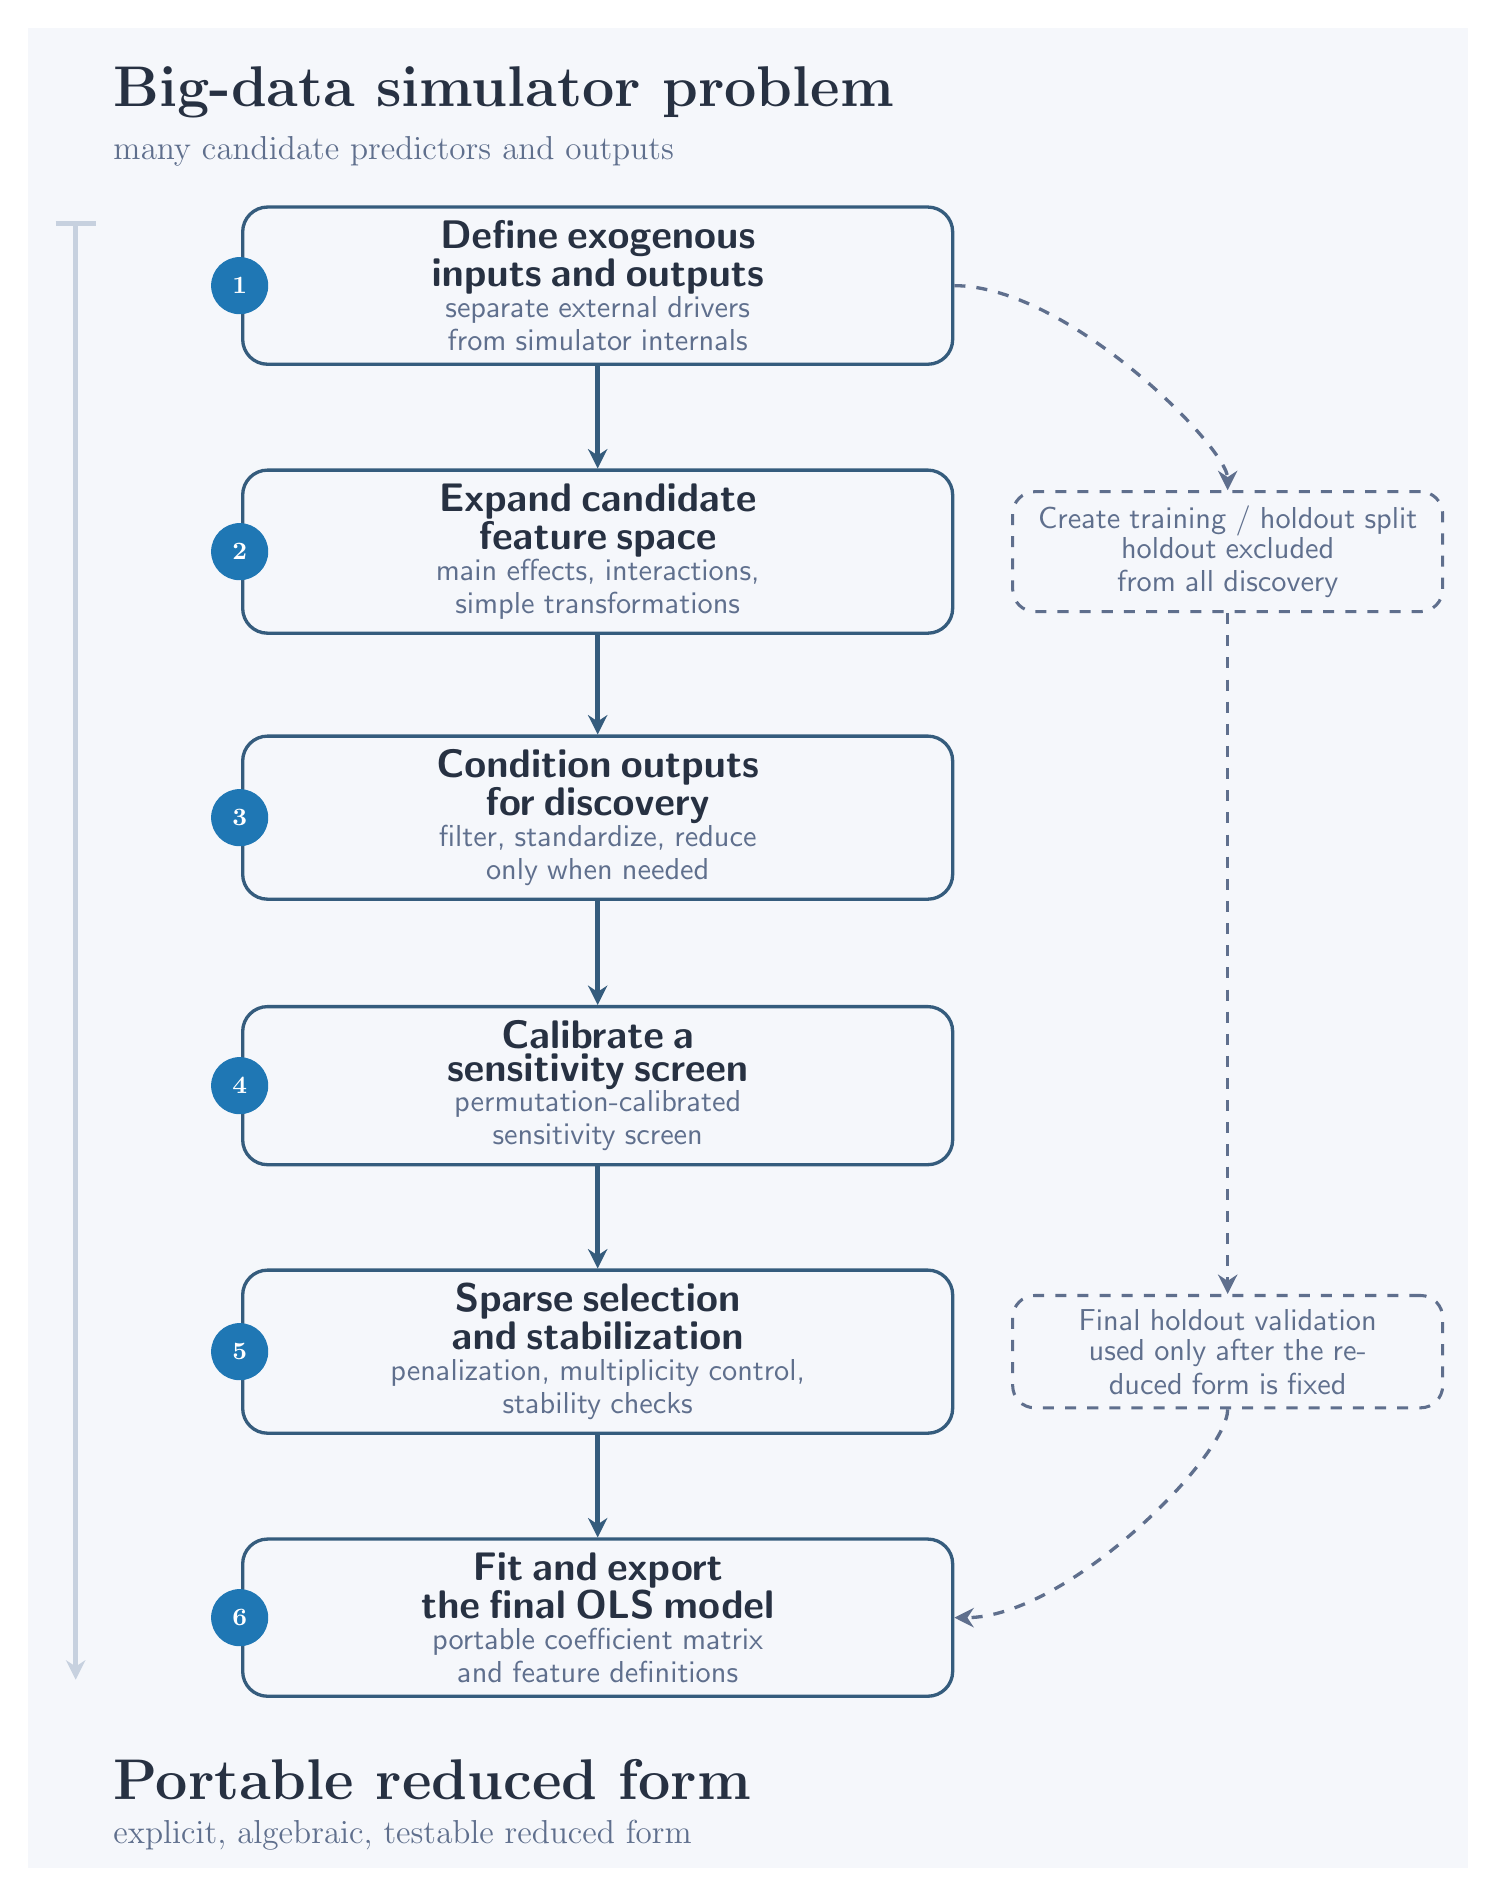
\begin{tikzpicture}[x=1in,y=1in,>=Stealth,font=\sffamily]

% canvas
\fill[figbg] (0,0) rectangle (7.20,9.20);

% header
\node[anchor=west,text=figdark,font=\bfseries\fontsize{20}{22}\selectfont]
  at (0.38,8.88) {Big-data simulator problem};
\node[anchor=west,text=figmid,font=\fontsize{12}{14}\selectfont]
  at (0.38,8.58) {many candidate predictors and outputs};

% footer
\node[anchor=west,text=figdark,font=\bfseries\fontsize{20}{22}\selectfont]
  at (0.38,0.44) {Portable reduced form};
\node[anchor=west,text=figmid,font=\fontsize{12}{14}\selectfont]
  at (0.38,0.16) {explicit, algebraic, testable reduced form};

% left guide — top flush with b1.north (8.22), bottom flush with b6.south (0.94)
\draw[figlight,line width=1.8pt] (0.24,8.22) -- (0.24,1.10);
\draw[figlight,line width=1.8pt] (0.14,8.22) -- (0.34,8.22);
\draw[figlight,line width=1.8pt,-{Stealth[length=7pt,width=7pt]}]
  (0.24,1.10) -- (0.24,0.94);

\tikzset{
  stage/.style={
    draw=figedge,
    fill=figbg,
    rounded corners=9pt,
    line width=1.2pt,
    minimum width=3.55in,
    minimum height=0.62in,
    text width=3.05in,
    align=center,
    inner sep=5pt
  },
  hold/.style={
    draw=figmid,
    fill=figbg,
    rounded corners=8pt,
    dash pattern=on 4pt off 4pt,
    line width=1.1pt,
    minimum width=2.15in,
    minimum height=0.52in,
    text width=1.95in,
    align=center,
    inner sep=5pt
  },
  badge/.style={
    circle,
    draw=figblue,
    fill=figblue,
    minimum size=0.28in,
    inner sep=0pt,
    text=white,
    font=\bfseries\small
  },
  mainflow/.style={
    draw=figedge,
    line width=1.6pt,
    -{Stealth[length=7pt,width=7pt]}
  },
  holdflow/.style={
    draw=figmid,
    dash pattern=on 4pt off 4pt,
    line width=1.2pt,
    -{Stealth[length=7pt,width=7pt]}
  }
}

% main boxes — 6 steps, x=2.85, step=1.332 from cy=7.91 to cy=1.25
% equal 0.28in white space above b1.top (8.22) and below b6.bot (0.94)
\node[stage] (b1) at (2.85,7.91)
  {\textcolor{figdark}{\bfseries\fontsize{14}{15}\selectfont Define exogenous\\inputs and outputs}\\[-1pt]
   \textcolor{figmid}{\fontsize{11}{12}\selectfont separate external drivers\\from simulator internals}};

\node[stage] (b2) at (2.85,6.58)
  {\textcolor{figdark}{\bfseries\fontsize{14}{15}\selectfont Expand candidate\\feature space}\\[-1pt]
   \textcolor{figmid}{\fontsize{11}{12}\selectfont main effects, interactions,\\simple transformations}};

\node[stage] (b3) at (2.85,5.25)
  {\textcolor{figdark}{\bfseries\fontsize{14}{15}\selectfont Condition outputs\\for discovery}\\[-1pt]
   \textcolor{figmid}{\fontsize{11}{12}\selectfont filter, standardize, reduce\\only when needed}};

\node[stage] (b4) at (2.85,3.91)
  {\textcolor{figdark}{\bfseries\fontsize{14}{15}\selectfont Calibrate a\\sensitivity screen}\\[-1pt]
   \textcolor{figmid}{\fontsize{11}{12}\selectfont permutation-calibrated\\sensitivity screen}};

\node[stage] (b5) at (2.85,2.58)
  {\textcolor{figdark}{\bfseries\fontsize{14}{15}\selectfont Sparse selection\\and stabilization}\\[-1pt]
   \textcolor{figmid}{\fontsize{11}{12}\selectfont penalization, multiplicity control,\\stability checks}};

\node[stage] (b6) at (2.85,1.25)
  {\textcolor{figdark}{\bfseries\fontsize{14}{15}\selectfont Fit and export\\the final OLS model}\\[-1pt]
   \textcolor{figmid}{\fontsize{11}{12}\selectfont portable coefficient matrix\\and feature definitions}};

% number badges
\foreach \n/\y in {1/7.91,2/6.58,3/5.25,4/3.91,5/2.58,6/1.25}{
  \node[badge] at (1.06,\y) {\n};
}

% main arrows
\draw[mainflow] (b1.south) -- (b2.north);
\draw[mainflow] (b2.south) -- (b3.north);
\draw[mainflow] (b3.south) -- (b4.north);
\draw[mainflow] (b4.south) -- (b5.north);
\draw[mainflow] (b5.south) -- (b6.north);

% holdout lane — h1 aligned with b2 (6.58), h2 aligned with b5 (2.58)
\node[hold] (h1) at (6.00,6.58)
  {\textcolor{figmid}{\fontsize{10.5}{11.5}\selectfont Create training / holdout split}\\[-1pt]
   \textcolor{figmid}{\fontsize{10.5}{11.5}\selectfont holdout excluded from all discovery}};

\node[hold] (h2) at (6.00,2.58)
  {\textcolor{figmid}{\fontsize{10.5}{11.5}\selectfont Final holdout validation}\\[-1pt]
   \textcolor{figmid}{\fontsize{10.5}{11.5}\selectfont used only after the reduced form is fixed}};

% holdout connectors
\draw[holdflow]
  (b1.east)
  .. controls (5.20,7.91) and (6.00,7.10) ..
  (h1.north);

\draw[holdflow]
  (h1.south) -- (h2.north);

\draw[holdflow]
  (h2.south)
  .. controls (6.00,2.06) and (5.20,1.25) ..
  (b6.east);

\end{tikzpicture}%
}
\caption{Reproducible workflow for constructing an interpretable reduced-form surrogate from a large simulator. The main vertical pipeline defines the external problem, expands a candidate feature space, conditions the output space, screens effects with permutation-calibrated sensitivity measures, performs sparse reduction, and ends in an exportable ordinary least squares reduced form. A separate holdout lane is reserved before any screening or selection step and is used only for final validation.}
\label{fig:workflow-generic-vertical}
\end{figure}

\section{Workflow}
\label{sec:workflow}

Figure~\ref{fig:workflow-generic-vertical} summarizes the workflow as a six-stage reduction pipeline with a separate holdout lane. The holdout split is created immediately after the external interface is defined and is not touched again until final validation. All standardization, filtering, feature discovery, selection, and final estimation are fit on the training sample only.

\begin{table}[p]
\centering
\caption{Reduced-form workflow corresponding to Figure~\ref{fig:workflow-generic-vertical}.}
\label{tab:algorithm-workflow}
\begin{tabular}{p{0.08\linewidth}p{0.32\linewidth}p{0.50\linewidth}}
\hline
Step & Operation & Output artifact \\
\hline
1 & Define exogenous inputs and target outputs. & External simulator interface $(U,Y)$, with simulator-internal states excluded unless they are explicit targets. \\
Holdout & Split training and validation rows. & Training rows for all adaptive modeling and a reserved holdout set used only after the final reduced form is fixed. \\
2 & Define and expand the candidate feature space. & Algebraic feature rules and, as screening/discovery proceeds, a materialized design matrix containing retained first-order terms plus discovered pairwise products and one-variable transformations. \\
3 & Condition outputs for discovery. & Train-standardized outputs, filtered outputs for discovery, and optional reduced response coordinates such as PCA scores. \\
4 & Calibrate a sensitivity screen. & Permutation-calibrated retained input set or retained candidate set; this stage is permissive and not treated as final inference. \\
5 & Perform sparse selection and stabilization. & Selected feature support based on enriched terms, penalized support recovery, multiplicity control, and stability diagnostics. \\
6 & Fit and export the final OLS model. & Standardized-scale OLS coefficients, raw-scale coefficient bundle, preprocessing vectors, metadata, and holdout validation summaries. \\
\hline
\end{tabular}
\end{table}

\subsection{Define exogenous inputs and outputs}

The workflow begins by defining the external interface to be approximated. The analyst identifies the exogenous drivers that will be varied outside the simulator and the outputs that matter for subsequent use. The target is a portable map from external drivers to reported outputs, not necessarily a reproduction of every simulator-internal state. At this stage the analyst also creates a training--holdout split. A holdout fraction $\eta_{\mathrm{hold}}$ in the range of roughly 5\%--20\% is a practical starting point, with 10\% often reasonable when the overall run count is large enough to support both discovery and validation. The holdout sample is excluded from every adaptive stage that follows.

\subsection{Expand candidate feature space}

The next step defines the algebraic candidate library for the external inputs. A practical starting library contains first-order terms, scientifically plausible pairwise products, and a restricted set of simple one-variable transformations, but the full cross-product library need not be materialized before screening. The library should be broad enough to capture interaction and curvature effects, but constrained so that every retained term can later be written down and evaluated directly. This is the stage at which the workflow commits to algebraic portability: even when later diagnostics use flexible models, candidate terms are restricted to forms that can appear in the final exported surrogate.

\subsection{Condition outputs for discovery}

The response side is conditioned in parallel. Let $Y_{\cdot m}$ denote scalar output $m$ across runs. Outputs with variance below a problem-specific floor $\varepsilon_{\mathrm{var}}$ are removed as structural zeros or near-deterministic quantities. We also filter outputs with negligible variation relative to scale using
\[
\mathrm{SNR}_m = \frac{\mathrm{Var}(Y_{\cdot m})}{\mathbb{E}(Y_{\cdot m}^2) + \delta},
\]
where $\delta > 0$ is a small numerical-stability constant (in the BSM implementation, $\delta = 10^{-10}$). All statistics are computed on training rows only; the holdout is not consulted at this stage. A practical starting rule is to remove outputs with $\mathrm{SNR}_m < \varepsilon_{\mathrm{snr}}$, with $\varepsilon_{\mathrm{snr}} \approx 10^{-2}$ serving as a useful default when outputs with negligible variation would otherwise dominate computational cost. When $p$ is too large for direct discovery, the standardized response matrix can be reduced temporarily to $r$ coordinates by a deterministic operator $\mathcal{R}$. If $\mathcal{R}$ is PCA, $r$ can be chosen to capture a target fraction $\tau_{\mathrm{PCA}}$ of retained output variance. The reduced response coordinates are used only for intermediate discovery and support recovery.

\subsection{Screen with a calibrated null}

The first major reduction step is a deliberately permissive screen calibrated against a null reference. In the BSM implementation, the screen used the moment-independent Delta sensitivity measure \citep{Borgonovo2007}. The analysis scripts compute Delta separately for each output and candidate input using aligned training data. For each null replicate, response rows are randomly reassigned relative to the input matrix, Delta values are recomputed, and the maximum Delta across inputs is retained for each output. The 95th percentile of this output-wise maximum null distribution provides a family-wise cutoff for that output. An input is retained when it exceeds the cutoff for at least one output. This screen is intentionally permissive: it controls the maximum-null comparison within each output, but does not claim global family-wise error control across all retained input--output pairs. Its role is to remove evidently negligible drivers before more expensive modeling while reducing the risk of early false exclusions.

More generally, the same role can be filled by any inexpensive multivariate or output-wise screen whose statistic is calibrated under an explicit null. If Monte Carlo permutation $p$-values are used, the usual finite-sample correction is
\[
\widehat p_j =
\frac{1 + \sum_{b=1}^{N_{\mathrm{perm}}}\mathbf{1}\{T_j^{(b)} \geq T_j^{\mathrm{obs}}\}}
{N_{\mathrm{perm}} + 1},
\]
where $T_j^{\mathrm{obs}}$ is the observed screening statistic and $T_j^{(b)}$ is the corresponding statistic under null replicate $b$. The BSM scripts used $N_{\mathrm{perm}}=200$, a 5\% family-wise maximum cutoff, and train-only standardized data products after the holdout split. % TODO-VERIFY: Recheck $N_{\mathrm{perm}}$, cutoff, and whether the final null implementation uses strict without-replacement permutation or random-index resampling against null_distribution.py, null_distribution.sh, and the final pipeline logs before submission.

\subsection{Discover interactions, curvature, and sparse support}

The screened set is enriched before final support recovery. Interaction candidates can be prioritized by fitting tree-based models to reduced response coordinates and computing SHAP interaction values. Tree-based SHAP methods provide polynomial-time explanations for tree ensembles and include interaction values that decompose prediction contributions into main and pairwise terms \citep{LundbergEtAl2020TreeSHAP}; the underlying SHAP framework is due to \citet{LundbergLee2017}. In the BSM case study, interaction strengths were aggregated across retained PCA scores and compared with a high permutation-null quantile. Nonlinear main effects were flagged with generalized additive model diagnostics \citep{HastieTibshirani1990}; when curvature was detected, the smooth term was approximated with the best-fitting member of a restricted algebraic library, such as quadratic, logarithmic, inverse, or exponential transforms.

The screened and enriched terms are then combined into an updated predictor matrix $X^{(1)}$. Sparse support recovery is carried out on the reduced response coordinates rather than directly on all scalar outputs. The BSM implementation used a multi-task elastic-net path with the selected tuning point at the LASSO endpoint, choosing the penalty by the extended Bayesian information criterion \citep{ChenChen2008}. The selected penalty used $\gamma_{\mathrm{EBIC}}=0.5$, which penalizes model size more strongly than ordinary BIC in large candidate spaces. Because selected supports can change with sample size and resampling variation, the workflow records stability diagnostics such as overlap of selected supports and rank agreement of coefficient magnitudes; these diagnostics are motivated by the same concern as stability-selection procedures \citep{MeinshausenBuhlmann2010}.

% TODO-VERIFY: Confirm the de-biased LASSO assumptions and exact filtering rule against LASSO_to_OLS_v9.ipynb and multivariate_mmreg_pipeline.with_subset.py. If the final repo does not document the assumptions sufficiently, retain the current conservative wording and avoid inferential claims.
The BSM support-recovery stage also applied nodewise LASSO \citep{MeinshausenBuhlmann2006} to estimate the inverse covariance structure of the selected predictors, yielding de-biased coefficient estimates with asymptotic normality \citep{ZhangZhang2014,VanDeGeerEtAl2014}. The analysis scripts applied Benjamini--Hochberg false-discovery-rate control \citep{BenjaminiHochberg1995} row-wise across PCA-score coefficients for each candidate predictor; a predictor was retained when at least one de-biased PCA-score coefficient survived this row-wise screen. This de-biasing step is used as a support-recovery selection device on PCA scores; it is not treated here as proof of valid post-selection inference for the full adaptive pipeline. We therefore do not make final output-wise significance claims for the exported OLS coefficient matrix.

\subsection{Fit and export the final OLS model}

Once the support set $S$ is fixed, the workflow returns from the reduced response representation to the full scalar output matrix. The final reduced form is estimated by unpenalized multivariate ordinary least squares on train-standardized $Y$ using train-standardized selected columns $\widetilde{X}_S$ and an intercept. Holdout predictions are inverse-transformed to the original output scale before validation metrics and plots are computed. This refit removes shrinkage from the support-recovery stage and yields a direct coefficient matrix that can be exported either on the standardized scale or as an equivalent raw-scale coefficient bundle. Ordinary least squares is used deliberately: not because the simulator is assumed to be globally linear in the raw inputs, but because the selected algebraic feature map makes a transparent and portable final representation possible.

Final validation is performed only once, on the holdout sample reserved at the beginning of the workflow. Predictive performance can be summarized with normalized root mean squared error or related scale-adjusted metrics, while interpretation is tied to the retained algebraic terms themselves rather than to latent variables or local explanation maps. The exported model consists of the input and output definitions, preprocessing rules, selected feature definitions, intercept vector, coefficient matrix, and supporting metadata needed to evaluate the reduced form outside the original simulator environment.

\section{Case Study: Bioenergy Scenario Model}
\label{sec:case}

The Bioenergy Scenario Model (BSM) provides the motivating application for the workflow and is used here as a demanding statistical test case. The BSM is a deterministic system dynamics model developed at the National Renewable Energy Laboratory to represent the biomass-to-biofuels supply chain and study U.S. biofuels deployment over multiple decades \citep{PetersonEtAl2013,LinEtAl2013BSMDocumentation}. In this article, model error refers to surrogate approximation error relative to deterministic BSM outputs, not to stochastic simulator noise. The value of the case study is methodological: BSM is rich enough to generate many coupled outputs, yet complex enough that repeated direct use can be cumbersome in subsequent studies.

For the present study, we impose explicit input and output boundaries before any statistical modeling begins. The input side is restricted to 160 exogenous drivers: 158 scalar inputs plus two binary variables treated as scenario switches. The output side is restricted to 635 annual time-series quantities selected for downstream relevance, each recorded annually from 2015 through 2051, yielding 23,495 scalar responses after flattening. The objective is not to emulate every internal state of BSM, but to construct a reduced form for a clearly defined external interface between exogenous drivers and reported outputs.

Simulation runs were generated from Latin hypercube designs over the scalar exogenous inputs \citep{McKayEtAl1979}. The two binary inputs define four scenario combinations. The first switch, \texttt{FM.Use Agnostic FS Conversion}, toggles whether agnostic herbaceous and woody feedstocks are usable by all modeled conversion processes rather than being targeted to specific pathways. The second switch, \texttt{OI.Use AEO Reference Oil}, toggles use of the Annual Energy Outlook reference oil-price projection rather than the corresponding high-price projection. We sampled all four combinations of these switches: both off, feedstock-conversion agnostic on only, reference-oil on only, and both on. Within each binary combination, 5,000 Latin hypercube samples were generated over the remaining 158 scalar inputs, giving $n=20,000$ simulator runs. A deterministic 10\% holdout split was then created with random seed 123, producing 18,000 training runs and 2,000 holdout runs. % TODO-VERIFY: LASSO_to_OLS_v9.ipynb appears to use a simple random holdout split rather than explicit scenario-stratified splitting; verify the final public pipeline and report per-scenario holdout counts before submission. The holdout sample was removed before standardization, output filtering, PCA fitting, sensitivity screening, SHAP interaction discovery, GAM curvature discovery, LASSO tuning, de-biased support recovery, and final OLS estimation.

The BSM documentation report provides the underlying model-data reference for interpreting the scenario inputs, target variables, units, and supply-chain modules \citep{LinEtAl2013BSMDocumentation}. The two binary variables are treated here as part of the external experimental design, while the remaining sampled inputs represent documented scalar assumptions such as incentive multipliers, incentive durations, conversion yields, fixed capital investment multipliers, operating-cost multipliers, required rates of return, commercial maturity indices, and progress ratios.

% TODO-VERIFY: Confirm support-recovery and final-export counts against final generated artifacts, especially selected_input_metadata, exported feature list, and coefficient bundle.
The support-recovery matrix in this case study contained 352 columns after screening and feature discovery: 63 first-order predictors, 248 second-order interaction terms, and 41 one-variable transformations. These are case-study counts for the implemented design matrix, not generic workflow constants. The initial 160-input interface was reduced because the calibrated Delta screen and subsequent feature-discovery stages removed inputs and derived terms that did not show sufficient evidence of association in the training data. The final LASSO support-recovery stage selected 346 features; the final OLS export retained 340 predictors after dropping zero-variance selected predictors in the training data. The retained OLS support comprised 61 main-effect terms, 242 pairwise interactions, and 37 one-variable transformations, representing 62 unique original inputs because some original inputs appear only through interactions or transformations.

% TODO-VERIFY: Confirm output culling counts and PCA retention target against LASSO_to_OLS_v9.ipynb, nonlinearity_check.ipynb, and final culling report.
The output-conditioning step used train-only standardization. Outputs with negligible variance or signal-to-noise ratio were removed for the PCA-based support-recovery stage. In the final LASSO notebook, the culling report retained 9,782 outputs and culled 13,713 outputs before PCA, with PCA configured to retain 95\% of the filtered output variance. This introduces a real risk: rare but scientifically important output-specific signals could be excluded from support recovery if they are removed by culling or represented weakly in the retained PCA scores. We mitigate this risk by using permissive output-filtering thresholds, retaining 95\% of filtered-output variance, using the reduced coordinates only for support recovery, and fitting the final OLS model against all 23,495 scalar outputs. The risk is not unique to PCA; basis reduction is a standard tool for high-dimensional simulator outputs \citep{HigdonGattikerWilliamsRightley2008}, but it must be treated as a computational approximation rather than as a guarantee that every output-specific signal is preserved.

\begin{table}[t]
\centering
\caption{Implementation constants for the BSM case study. Working values are drawn from the current analysis scripts and notebooks for the reported workflow; items marked with in-source TODO comments require final verification against the public-release artifacts before submission.}
\label{tab:implementation-constants}
\begin{tabular}{lll}
\hline
Quantity & Value & Use \\
\hline
Total simulator runs & 20,000 & full sampled design \\ % TODO-VERIFY: confirm against sample manifest/final run inventory
Scalar sampled inputs & 158 & Latin hypercube dimensions within scenario \\ % TODO-VERIFY: confirm against input metadata/exported sample design
Binary scenario inputs & 2 & four scenario combinations \\ % TODO-VERIFY: confirm exact switch names in public metadata
Runs per scenario combination & 5,000 & scenario-balanced design \\ % TODO-VERIFY: confirm per-combination counts after dropped/failed runs
Holdout fraction & 10\% & external validation \\
Training runs & 18,000 & all adaptive modeling and final fit \\
Holdout runs & 2,000 & final validation only \\
Random seed & 123 & holdout split and repeated stochastic choices \\ % TODO-VERIFY: confirm every stochastic stage that used this seed
Delta null replicates & 200 & empirical null calibration \\ % TODO-VERIFY: confirm against null_distribution.py and final logs
Delta internal resamples & 100 & SALib Delta confidence/resampling setting \\ % TODO-VERIFY: confirm whether final pipeline changes SALib num_resamples
Delta cutoff & 5\% output-wise maximum-null cutoff & permissive screen before feature discovery \\
Output variance floor & $10^{-8}$ & near-zero-variance culling \\ % TODO-VERIFY: confirm against output-filtering code
SNR threshold & $10^{-2}$ & low-signal output culling \\ % TODO-VERIFY: confirm against output-filtering code
PCA variance target & 95\% & reduced response coordinates \\ % TODO-VERIFY: nonlinearity_check.ipynb/FY25Q4 report mention 90%; final LASSO notebook appears to use 95%
LASSO subset size & 3,000 & final PCA-score support recovery \\ % TODO-VERIFY: confirm final production subset size
EBIC $\gamma$ & 0.5 & penalized-model selection \\ % TODO-VERIFY: confirm final EBIC configuration
FDR threshold & 0.05 & de-biased coefficient screen on PCA scores \\ % TODO-VERIFY: confirm final multiplicity correction threshold
Stability Jaccard threshold & 0.75 & support overlap across resampled subsets \\
Stability Spearman threshold & 0.90 & coefficient rank agreement across subsets \\
nRMSE range floor & $10^{-6}$ & exclude zero-range outputs from macro nRMSE \\ % TODO-VERIFY: confirm against metric function used for reported values
\hline
\end{tabular}
\end{table}

\section{Results}
\label{sec:results}

\subsection{Reduction of predictor and output complexity}

% TODO-VERIFY: Confirm per-type predictor counts against the exported selected_input_metadata artifact, final feature-definition table, and final coefficient bundle from the canonical production run. The current working numbers are 352 enriched columns = 63 first-order + 248 interaction + 41 transformation; 346 LASSO-selected features; and 340 final OLS predictors = 61 main-effect + 242 interaction + 37 transformation, representing 62 unique original inputs.
The workflow reduced both sides of the statistical problem. On the predictor side, the implemented enriched design matrix contained 352 columns after screening and feature discovery: 63 first-order terms, 248 pairwise interaction terms, and 41 one-variable nonlinear transformations. The de-biased LASSO support-recovery step selected 346 features, and the final OLS export retained 340 predictors after training-set zero-variance checks. The retained OLS support contained 61 main-effect terms, 242 pairwise interactions, and 37 one-variable transformations, representing 62 unique original inputs.

On the response side, the simulator output interface contained 23,495 scalar responses. Intermediate support recovery used standardized, filtered outputs and PCA scores as a computational device. The final OLS solve used train-standardized full outputs and train-standardized selected predictors, and predictions were inverse-transformed to the original output scale for evaluation and release. This distinction matters: the PCA scores are not the released prediction target, and the final validation metrics are computed on raw-scale BSM outputs.

\begin{table}[t]
\centering
\caption{Stagewise reduction summary for the BSM reduced form. Counts describe the implemented predictor and response reductions used to produce the exported surrogate.}
\label{tab:results-summary}
\begin{tabular}{lll}
\hline
Quantity & Value & Role in workflow \\
\hline
Simulator runs & 20,000 & full sampled design \\ % TODO-VERIFY: final run inventory
Training runs & 18,000 & all adaptive modeling stages \\ % TODO-VERIFY: holdout split artifact
Holdout runs & 2,000 & final external validation only \\ % TODO-VERIFY: holdout split artifact
Exogenous inputs & 160 & external driver set \\ % TODO-VERIFY: input metadata
Scalar responses & 23,495 & final multivariate prediction target \\ % TODO-VERIFY: output metadata
Enriched predictors after screening/discovery & 352 & support-recovery design matrix \\ % TODO-VERIFY: final enriched design matrix columns
First-order terms in enriched matrix & 63 & main-effect terms before final support recovery \\ % TODO-VERIFY: enriched metadata
Second-order terms in enriched matrix & 248 & pairwise interaction terms before final support recovery \\ % TODO-VERIFY: enriched metadata
One-variable transformations in enriched matrix & 41 & transformed terms before final support recovery \\ % TODO-VERIFY: enriched metadata
Filtered outputs for PCA support recovery & 9,782 & retained by train-only culling \\ % TODO-VERIFY: output culling report
Culled outputs for PCA support recovery & 13,713 & removed from PCA stage only \\ % TODO-VERIFY: output culling report
PCA retention target & 95\% & filtered-output variance target \\ % TODO-VERIFY: reconcile with 90% references in earlier artifacts
LASSO-selected features & 346 & support-recovery output \\ % TODO-VERIFY: LASSO output artifact
Final retained OLS predictors & 340 & exported algebraic support \\ % TODO-VERIFY: final OLS export
Final retained main-effect terms & 61 & direct main-effect terms in exported support \\ % TODO-VERIFY: final OLS metadata
Final retained interaction terms & 242 & pairwise products in exported support \\ % TODO-VERIFY: final OLS metadata
Final retained transformation terms & 37 & one-variable transformations in exported support \\ % TODO-VERIFY: final OLS metadata
Unique original inputs represented & 62 & original inputs appearing as main effects, interactions, or transformations \\ % TODO-VERIFY: derived from final support metadata
\hline
\end{tabular}
\end{table}

\subsection{Predictive fidelity on unseen simulator runs}

Predictive performance was assessed only on the fixed 2,000-run holdout sample reserved before screening, discovery, selection, and estimation. The normalized root mean squared error reported here is the macro-average of output-wise RMSE values normalized by the corresponding training-set output ranges. Let $H$ denote holdout rows, $T$ denote training rows, and let
\[
\mathcal{M}=\left\{m: \max_{i\in T}Y_{im} - \min_{i\in T}Y_{im} \geq 10^{-6}\right\}
\]
be the set of outputs with non-negligible training range. The reported metric is
\[
\mathrm{nRMSE}_{\mathrm{macro}}
= \frac{1}{|\mathcal{M}|}
\sum_{m\in\mathcal{M}}
\frac{
\left[|H|^{-1}\sum_{i\in H}\left(Y_{im}-\widehat{Y}_{im}\right)^2\right]^{1/2}
}{
\max_{i\in T}Y_{im}-\min_{i\in T}Y_{im}
}.
\]
% TODO-VERIFY: Confirm nRMSE implementation and row-bootstrap procedure against LASSO_to_OLS_v9.ipynb and final metrics code.
A row-bootstrap confidence interval for this macro nRMSE can be constructed by resampling holdout rows while holding the trained model and training-set normalization ranges fixed; the resulting interval values will be reported once confirmed from the final pipeline.

Using this definition, the intermediate penalized model achieved holdout macro nRMSE 0.0859, and the final OLS refit achieved holdout macro nRMSE 0.0445.
% TODO-VERIFY: Confirm both metrics against final validation summary; do not submit until generated from the public-release pipeline.
The improvement is consistent with the intended role of the final refit: the penalized model is used for support recovery on reduced response coordinates, whereas the exported model is an unpenalized fit on the full output matrix.

The current validation evidence is intentionally narrower than a full model-card-style audit. The manuscript reports the external holdout macro nRMSE, the reduction in predictor and output complexity, and the structure of the retained support. Those results support the narrower workflow claim advanced here: the staged reduction pipeline can produce an explicit algebraic surrogate with low average holdout macro nRMSE. More detailed ablation studies and output-wise error diagnostics are marked as final verification targets and should be added once their generated tables are part of the public-release evidence bundle.

\subsection{Structure of retained effects}

The retained support is best interpreted as an explicit algebraic index set rather than as a hand-readable coefficient table. The final coefficient matrix contains one coefficient per retained predictor and scalar response, plus output-specific intercepts. With 340 retained predictors and 23,495 scalar responses, this is still a large matrix. The interpretability claim is therefore structural: the feature support is finite, named, algebraic, and auditable; the full coefficient matrix is exportable and queryable.

The retained feature composition indicates that the reduced form depends on more than isolated main effects. Pairwise interaction terms account for most retained predictors, while main-effect and one-variable nonlinear terms remain present. Figure~\ref{fig:results-feature-composition} shows the breakdown of the retained support by term type. This supports the design choice to discover and carry forward interactions and curvature before final OLS refitting. It also shows why a purely main-effects reduced form would be a weak default for this simulator.

Figure~\ref{fig:results-interaction-density} shows the distribution of retained interaction pairs by BSM module pair. Note that this figure shows raw retained counts, not opportunity-normalized interaction rates; modules with more candidate inputs accumulate higher counts for structural reasons. The full retained pair list is in the supplementary bundle.

% TODO-VERIFY: Confirm feature-composition counts in this figure against final exported support metadata and Table~\ref{tab:results-summary}.
\begin{figure}[t]
\centering
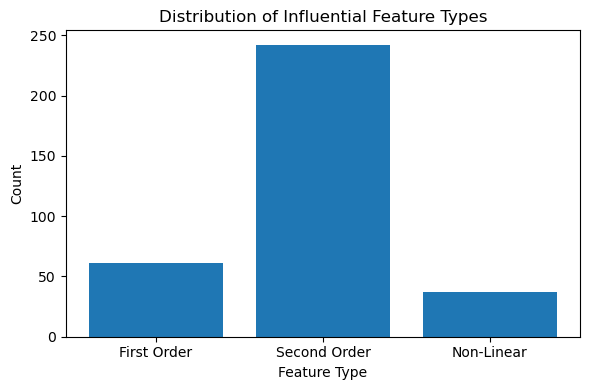
\includegraphics[width=0.72\linewidth]{results_feature_type_composition.png}
\caption{Composition of the retained predictor support by term type in the final reduced form. The final OLS export retained 340 predictors after training-set zero-variance checks: 61 main-effect terms, 242 pairwise interaction terms, and 37 one-variable nonlinear transformations. The de-biased LASSO support-recovery stage selected 346 features before that final export check. Interaction terms dominate the retained support, with main-effect and transformation terms still present.}
\label{fig:results-feature-composition}
\end{figure}

% TODO-VERIFY: Confirm interaction-module counts and whether the plotted values are raw counts or opportunity-normalized densities.
\begin{figure}[t]
\centering
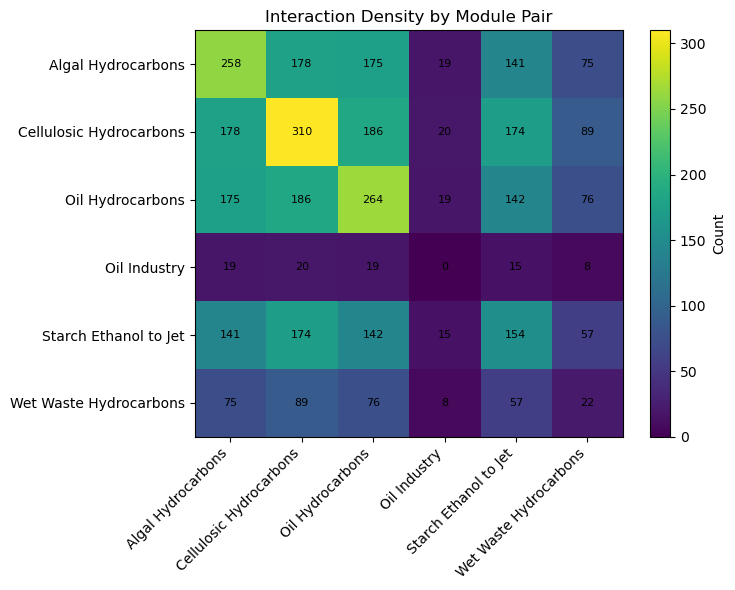
\includegraphics[width=0.82\linewidth]{results_interaction_density_heatmap.png}
\caption{Count matrix of retained second-order interaction terms by BSM module pair. Values are raw counts of retained interaction terms symmetrized across module pairs, not normalized by the number of candidate pairs available within each module pair. Modules with larger input sets can accumulate higher counts for structural reasons unrelated to interaction density. The full list of retained interaction pairs is provided in the supplementary artifact bundle.}
\label{fig:results-interaction-density}
\end{figure}

\subsection{Practical value of the final reduced form}

The workflow ends with an OLS intercept vector, coefficient matrix, selected feature definitions, input metadata, output metadata, and preprocessing rules, rather than with a software-bound emulator object. Together, these components define a reduced form that can be evaluated outside the original BSM environment and incorporated into subsequent studies that need an explicit approximation rather than repeated simulator execution.

Relative to a software-bound or otherwise opaque surrogate object, the reduced form provides a named algebraic support and an explicit coefficient matrix that can be inspected, versioned, and embedded in downstream analyses without requiring direct access to the original simulator.

\FloatBarrier

\section{Discussion}
\label{sec:discussion}

The BSM case study shows that a high-dimensional simulator interface can be reduced through a documented statistical workflow rather than by ad hoc manual term selection. In the reported run, the workflow converted 20,000 simulator evaluations with 160 exogenous inputs and 23,495 scalar responses into an exported OLS reduced form with 340 retained predictors derived from 62 unique original inputs. The central contribution is the combination of three properties: the final model remains accurate on an untouched holdout set under the reported macro nRMSE metric, the retained support is explicit and algebraic, and the exported object is portable outside the original simulator.

The workflow perspective matters because the underlying statistical tasks are heterogeneous. Interface definition, calibrated screening, structured feature discovery, sparse support recovery, final estimation, and external validation solve different problems and should not be collapsed into a single model-fitting step. The calibrated screen is deliberately permissive because its role is to remove evidently negligible drivers without making early irreversible exclusions. The reduced-response discovery stages are computational devices for exposing structure across a very large output collection. The final OLS refit serves a different purpose again: it removes shrinkage from support recovery and produces the coefficient bundle required for export.

The results should nevertheless be interpreted cautiously. First, the final surrogate is linear in the selected algebraic feature library, so higher-order nonlinearities, discontinuities, and regime changes can still be missed. Second, the screening and discovery stages can be computationally demanding, especially the permutation-calibrated Delta screen and SHAP interaction discovery. Third, the reduced form is validated on held-out runs drawn from the same experimental design, so the reported performance is best interpreted as within-design generalization rather than unrestricted extrapolative validity. Fourth, the evidence reported here is concentrated on macro holdout error and structural summaries of the retained support; richer output-wise diagnostics are still needed to show where the reduced form succeeds and fails across individual outputs, modules, and years. Fifth, this article does not present a head-to-head benchmark against alternative surrogate classes, so its claim is about the viability of the workflow, not about dominance over other modeling strategies.

Within those limits, the broader implication is practical. Interpretable reduced forms do not need to be restricted to hand-selected predictors if the reduction problem is staged carefully. Large simulator studies can be compressed into auditable surrogate models that support later prediction, scenario exploration, targeted sensitivity analysis, and downstream model integration without repeated direct simulator execution.

\section{Conclusion}
\label{sec:conclusion}

Staged statistical reduction provides a practical route from a high-dimensional simulator interface to an exportable reduced form. In the reported BSM case study, permutation-calibrated sensitivity screening, structured interaction and curvature discovery, sparse support recovery, and final OLS refitting produced an algebraic surrogate with holdout macro nRMSE 0.0445 under the reported metric while preserving an auditable input--output representation.

The main point is not that OLS is always sufficient for large simulators. It is that an explicit algebraic feature map, selected through a documented workflow and validated on an untouched holdout set, can turn a simulator-specific analysis into a reusable statistical object. That separation between simulator execution and statistical reduction is what makes the resulting approximation portable, inspectable, and testable outside the original modeling environment.

\section{Reproducibility and Released Artifacts}
\label{sec:reproducibility}

Reproducibility in this article is defined at the workflow-and-model level. The aim is to make the reduced-form construction auditable and reusable from the documented external interface, without requiring repeated execution of simulator internals that may not be portable outside the original modeling environment.

At the time of this revision, the public release identifiers for the repository and archived bundle were still pending. The planned release materials include the analysis scripts, notebooks, environment specification, exported reduced-form bundle, feature definitions, input metadata, output metadata, coefficient matrices, intercept vectors, validation summaries, and figure-generation code. The released bundle should include both standardized-scale and raw-scale coefficient products so that users can evaluate the surrogate directly from documented input values.

The reproducibility entry point should be documented in the repository README and cited here with the final release URL and DOI once available. The release workflow is expected to include installation of the locked computational environment, execution of the validation gate, regeneration of the reduced-form bundle from the released intermediate data products, and rebuilding of manuscript figures and summary tables. Large simulator raw-output files that cannot be redistributed should be replaced by documented derived artifacts sufficient to audit the statistical workflow and evaluate the exported reduced form.

\begin{esm}
\esmtitle{Supplementary Material}
\esmdescription{Supplementary material for this article is planned for the public repository and archived release. The supplement is expected to include the reduced-form bundle, input and output metadata, selected feature definitions, raw-scale and standardized coefficient matrices, validation summaries, figure-generation scripts, and reproducibility instructions.}
\esmfilename{bsm-public-rf-supplement.zip}
\end{esm}

\begin{appendix}

\section{Reduced-form scope and use limits}
\label{app:model-card}

\begin{table}[h]
\centering
\caption{Scope limits for applying the BSM reduced form.}
\label{tab:scope-limits}
\begin{tabular}{p{0.25\linewidth}p{0.65\linewidth}}
\hline
Item & Scope statement \\
\hline
Intended use & Fast approximation of the documented BSM external input--output interface within the sampled experimental design. \\
Primary output & Predictions for the 23,495 scalar responses formed from 635 annual time-series outputs over 2015--2051. \\
Input domain & The documented ranges of the 158 scalar sampled inputs and the four combinations of the two binary scenario inputs. \\
Required preprocessing & Apply the released feature definitions and standardization rules exactly, or use the raw-scale coefficient bundle provided in the release. \\
Validation domain & Held-out simulator runs drawn from the same scenario-balanced Latin hypercube design as the training data; final release should report holdout counts by binary scenario combination. \\
Invalid use & Extrapolation outside the sampled input ranges, replacement of BSM for structural model changes, or policy conclusions without checking the relevant full-simulator scenario. \\
Known limitations & Linear in the selected algebraic feature library; may miss higher-order interactions, discontinuities, and rare output-specific signals not represented in support recovery. \\
\hline
\end{tabular}
\end{table}

\section{Additional validation tables}
\label{app:validation-tables}

Detailed ablation results, output-wise error summaries, and module-level diagnostics are not included in this revision. They should be added once the corresponding validation runs are part of the final evidence bundle.
\end{appendix}

\begin{acknowledgement}%[title={Acknowledgments}]
% TODO-VERIFY: Replace acknowledgement text with final institution-approved wording before internal or journal submission.
The authors thank National Laboratory of the Rockies collaborators and internal reviewers whose technical feedback improved the workflow, implementation, and manuscript.
\end{acknowledgement}

\begin{funding}
% TODO-VERIFY: Replace with the required DOE/NREL award, contract, and disclaimer language approved for public release.
Funding was provided by the Bioenergy Technologies Office of the U.S. Department of Energy.
\end{funding}

\bibliographystyle{jds}
\bibliography{ref}

\end{document}
